\documentclass{article}
\usepackage[utf8]{inputenc}

\title{Relatório Web Semântica \\ \textbf{Domínio}: Agricultura}
\author{Romário Ferreira \& Elói Dreves Vieira}
\date{Quinta-feira, 31 de outubro de 2019}

\usepackage{natbib}
\usepackage{graphicx}

\begin{document}

\maketitle

\section{Introdução}
Este relatório tem como intuito relatar o assunto estudado na logica descritiva e a implementação 
de um domínio com caso de estudo. O objetivo deste relatório é mostrar como ocorreu a solução do problema em estudo e bem como apresentar os resultados obtidos ao aplicar o problema no software 
\textit{protegé}, assim sendo adotou-se o domínio para estudo como sendo Agricultura, pois bem, procurou-se escolher este domínio pois ele é conhecido e de fácil entendimento para os demais, e também ao realizar a modelagem da lógica descritiva não ocorrerem problemas desconhecimento do domínio.

Para implementação do domínio e representar a forma do conhecimento, utilizou-se o software como aliadado para realizar as inferências lógicas, neste contexto inseriu-se no software o Tbox 
\footnote{\textbf{tbox} descrevem uma conceitualização de um domínio de interesse}
e Abox \footnote{\textbf{ABox} são declarações compatíveis com tbox sobre indivíduos pertencentes a esses conjuntos.} descrevem uma conceitualização de um domínio de interesse.

Neste relatório abordou-se o estudo do domínio agricultural, desta forma aplicado a utilizando logica descritiva, permitindo-se a construção do tbox e abox, assim pode-se aplicar ao software protégé para melhor entendimento.


\section{Desenvolvimento}
    Para dar inicio ao estudo definimos o domínio como sendo Órgão público em especifico IBAMA, porém notamos dificuldades neste domínio e decidimos alterar-lo, assim sendo escolhemos outro domínio
    no qual é voltado a Agricultura, posteriormente decidimos realizar o tbox , assim observou-se o 
    domínio para coletar as informações necessárias para realização do mesmo.
    E com isso foi iniciado a produção da ontologia através do desenvolvimento dos conceitos, indivíduos e as propriedades que após diversas edições e modificações ficaram conforme as figuras apresentadas abaixo respectivamente.
    
    \begin{figure}[!htp]
        \centering % para centralizarmos a figura
        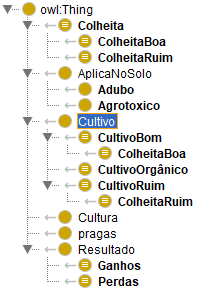
\includegraphics[width=.5\textwidth]{imagens/class.png} % leia abaixo
        \caption{Estrutura de normas de conceitos aplicadas ao domínio agricultural.}
        \label{figura:disjunt}
    \end{figure}
    
    \begin{figure}[!htp]
        \centering % para centralizarmos a figura
        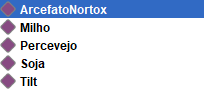
\includegraphics[width=.5\textwidth]{imagens/Individuos.png} % leia abaixo
        \caption{Lista de indivíduos inseridas no domínio agricultural.}
        \label{figura:disjunt}
    \end{figure}
    
    \begin{figure}[!htp]
        \centering % para centralizarmos a figura
        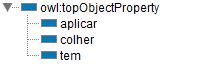
\includegraphics[width=.5\textwidth]{imagens/Properties.png} % leia abaixo
        \caption{Estrutura de objetos de propriedades disponíveis para uso no domínio agriculural.}
        \label{figura:disjunt}
    \end{figure}
    

\section{Inferências Obtidas com a ontologia }
    


   % Apesar da ontologia ser bastante enxuta ao dar inicio ao resolver e finalizar as edições foram obtidas diversas inferências.    

%    \textbf{A PARTIR DAQUI EDITAR CONFORME ARQUIVO DOC QUE ESTÁ NO GIT.}
    Apresenta-se inicialmente a classe que também é conhecida como normas de conceitos, neste caso, pode-se visualizar a norma de conceito de colheita e sua estrutura na imagem \ref{figura:descricaoColheta} e assim verificar quais foram as inferências geradas pelo motor de inferências, para este caso cultivo e resultados foram inferidos. Desta forma a norma de conceito tornou-se a subclasse de cultivo e resultado, devido a sua regra estar contida em um contexto, assim resultando duas inferências. 

    %A primeira a ser apresentada será a da colheita onde após ter sua regra especificada automaticamente houve a inferência me que ela se torna subclasse de Cultivo e Resultado, devido a sua regra apresentar Cultivo em alguma parte, que resultou nas duas inferências.
    
    \begin{figure}[!htp]
        \centering % para centralizarmos a figura
        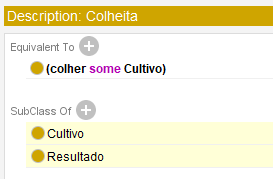
\includegraphics[width=.5\textwidth]{imagens/Inf_1.png} % leia abaixo
        \caption{Apresenta a descrição de uma colheita.}
        \label{figura:descricaoColheta}
    \end{figure}


    Assim foi criado duas subclasses para colheita a \textit{ColheitaBoa} e \textit{ColheitaRuim}, onde tiveram inferências a \textit{CultivoBom} e Ganhos no caso da \textit{ColheitaBoa} e no caso de \textit{ColheitaRuim} que teve inferência a \textit{CultivoRuim} e Perdas, no entanto ao especificar as regras não foram só obtidos as inferências como também elas passaram ser  automaticamente subclasses tanto de \textit{CultivoBom} quanto de \textit{CultivoRuim} como pode ser visto na Figura \ref{figura:descricaoColheta}.
    
    
    \begin{figure}[!htp]
        \centering % para centralizarmos a figura
        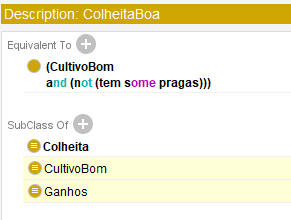
\includegraphics[width=.5\textwidth]{imagens/Inf_2.png} % leia abaixo
        \caption{Apresenta a descrição de uma colheita boa e as inferências realizadas pelo motor de inferência.}
        \label{figura:descricaoColhetaBoa}
    \end{figure}
    
     \begin{figure}[!htp]
        \centering % para centralizarmos a figura
        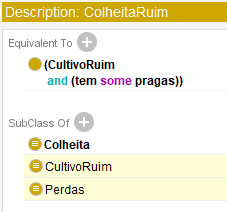
\includegraphics[width=.5\textwidth]{imagens/inf_3.png} % leia abaixo
        \caption{Apresenta a descrição de uma colheita ruim e as inferências.}
        \label{figura:descColhetaRuim}
    \end{figure}
    
    Em \textit{CultivoBom} e \textit{CultivoRuim} ambos tiveram a mesma inferência como subclasses de Resultado, porém \textit{CultivoBom} além desta inferência também teve a inferência ao indivíduo Soja devido a suas propriedades.
    
     \begin{figure}[!htp]
        \centering % para centralizarmos a figura
        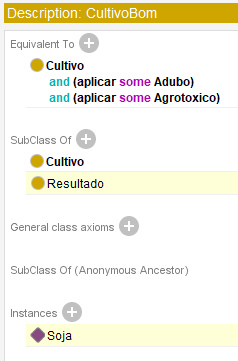
\includegraphics[width=.5\textwidth]{imagens/Inf_4.png} % leia abaixo
        \caption{Apresenta a descrição de um cultivo bom.}
        \label{figura:descCultivoBom}
    \end{figure}
     
     \begin{figure}[!htp]
        \centering % para centralizarmos a figura
        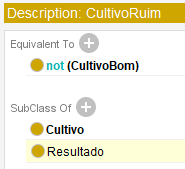
\includegraphics[width=.5\textwidth]{imagens/Inf_5.png} % leia abaixo
        \caption{Apresenta a descrição de um cultivo ruim.}
        \label{figura:descCultivoRuim}
    \end{figure}
    
     \begin{figure}[!htp]
        \centering % para centralizarmos a figura
        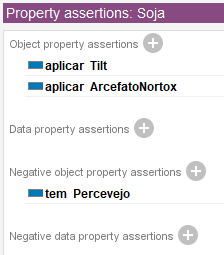
\includegraphics[width=.5\textwidth]{imagens/prop_soja.png} % leia abaixo
        \caption{Apresenta as propriedades da classe soja}
        \label{figura:descPropriedadeSoja}
    \end{figure}
    
    E também tivemos a inferência do \textit{CultivoOrganico} como subclasse de \textit{CultivoRuim}.
    
      \begin{figure}[!htp]
        \centering % para centralizarmos a figura
        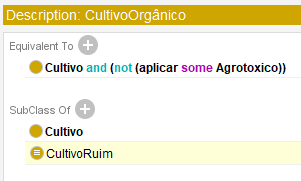
\includegraphics[width=.5\textwidth]{imagens/Inf_6.png} % leia abaixo
        \caption{Apresenta as descrição de cultivo orgânico}
        \label{figura:desc\textit{CultivoOrganico}}
    \end{figure}
    
    Além de Cultura e Pragas ambas terem inferência com Cultivo e Resultado.

  \begin{figure}[!htp]
        \centering % para centralizarmos a figura
        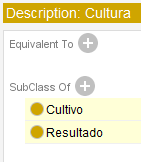
\includegraphics[width=.5\textwidth]{imagens/Inf_7.png} % leia abaixo
        \caption{Apresenta as descrição de cultura e as inferências ocorridas nesta classe}
        \label{figura:descCulturaInferencia}
    \end{figure}

    \begin{figure}[!htp]
        \centering % para centralizarmos a figura
        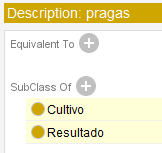
\includegraphics[width=.5\textwidth]{imagens/Inf_8.png} % leia abaixo
        \caption{Apresenta as descrição de pragas e as inferências ocorridas nesta classe, sendo tais cultivo e resultado.}
        \label{figura:descPragas}
    \end{figure}
    
    E por fim Ganhos e Perdas que tiveram inferência ao Cultivo e Perdas além desta também teve uma inferência ao indivíduo Milho devido a suas propriedades.
    
    \begin{figure}[!htp]
        \centering % para centralizarmos a figura
        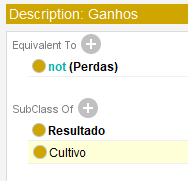
\includegraphics[width=.5\textwidth]{imagens/Inf_9.png} % leia abaixo
        \caption{Apresenta a equivalência da classe ganhos e sua inferências de cultivo}
        \label{figura:descGanhos}
    \end{figure}
    
    \begin{figure}[!htp]
        \centering % para centralizarmos a figura
        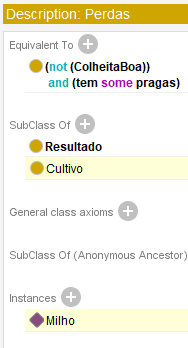
\includegraphics[width=.5\textwidth]{imagens/Inf_10.png} % leia abaixo
        \caption{Apresenta a equivalência da classe perdas e sua inferências com cultivo e milho}
        \label{figura:descPerdas}
    \end{figure}
    
    \begin{figure}[!htp]
        \centering % para centralizarmos a figura
        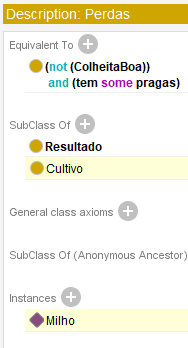
\includegraphics[width=.5\textwidth]{imagens/Inf_10.png} % leia abaixo
        \caption{Apresenta propriedade milho, onde foi informado que milho tem percevejo.}
        \label{figura:PropMilho}
    \end{figure}
    
    
\subsection{exemplos simbolos}    
Equivalencia = \equiv
SubClass = \sqsubseteq
AND = \sqcap
OR = \sqcup
Existe = \exists
Not = \neg

\subsection{Satisfatibilidade}
$CultivoBom \equiv Cultivo(soja) \sqcap aplicar(soja, tilt) \sqcap aplicar(soja, arcefatonortox)$ \\
\newline
\textbf{Adubo}(tilt) \\
\textbf{Agrotoxico}(ArcefatoNortox)

\subsection{Subsunção de conceito}
$CultivoBom \sqcap CultivoRuim \sqsubseteq Cultivo $ \\
\newline
\textbf{Classificador}: Cultivo \\
\textbf{Classificados}: CultivoBom, CultivoRuim

\subsection{Consequência lógica}
$CultivoBom \equiv Cultivo \sqcap \exists aplicar.Adubo \sqcap \exists aplicar.Agrotoxico$

\subsection{Equivalência entre conceitos}
$CultivoBom \equiv Cultivo \sqcap \exists aplicar.Adubo \sqcap \exists aplicar.Agrotoxico$ \\ \\
$CultivoRuim \equiv \neg CultivoBom$

\subsection{Consistência da ontologia}
$CultivoBom(Soja) \equiv Cultivo(Soja)$

\subsection{Checagem de instância}
$CultivoBom(Soja) \equiv Cultivo(Soja) \sqcap \exists aplicar.Adubo \sqcap \exists aplicar.Agrotoxico$

\section{Situações que reforçam o uso da
semântica de mundo aberto pelo motor de inferência subjacente}



\newpage

\section{Conclusão}
    Pode se compreender com este estudo que qualquer domínio pode-se utilizar-se para realizar inferências através de ontologias, assim definido o contexto de estudo, pode-se criar o tbox e abox, utilizando o auxílio de ferramentas para realizar inferências.
    
    Por meio do desenvolvimento e execução do domínio estudado no protegé, mesmo que o domínio agricultural em nosso estudo tenha sido aplicado de forma trivial, evidenciou-se e ficou claro o poder de dedução lógica do motor de infência utilizado por meios dos recursos disponíveis na web semântica.
    
    %Por meio da execução do domínio que foi passado ao protegé, neste caso uma ontologia trivial, evidenciou-se que é impressionante a percepção do poder de dedução lógica do motor de inferências da web semântica.
    
    Pudemos acompanhar os resultados apresentado pelo software assim, tivemos oportunidades de verificar problemas como base inconsistente ou ainda a disjunção de conjuntos.

\end{document}
